\chapter{Cucurrency}

\section{Cucurrency and Thread}

    Thread: very much like process, except threads share the same address space and thus
    can access the same data.

\ssc{Threads vs Processes}

\sssc{Similarities between Processes and Threads}

    A thread has a program counter(PC), own set of registers. When switching from
    thread T1 to thread T2, a context switch must take place. There would be 
    thread control blocks (TCB) like PCB to store the state of each thread.

\sssc{Difference between Processes and Threads}

    1. The address space of threads within a single process is the same.

    2. Multi-threaded Address Spaces has different structure: one stack per thread called
    \tbi{thread-local} storage.

    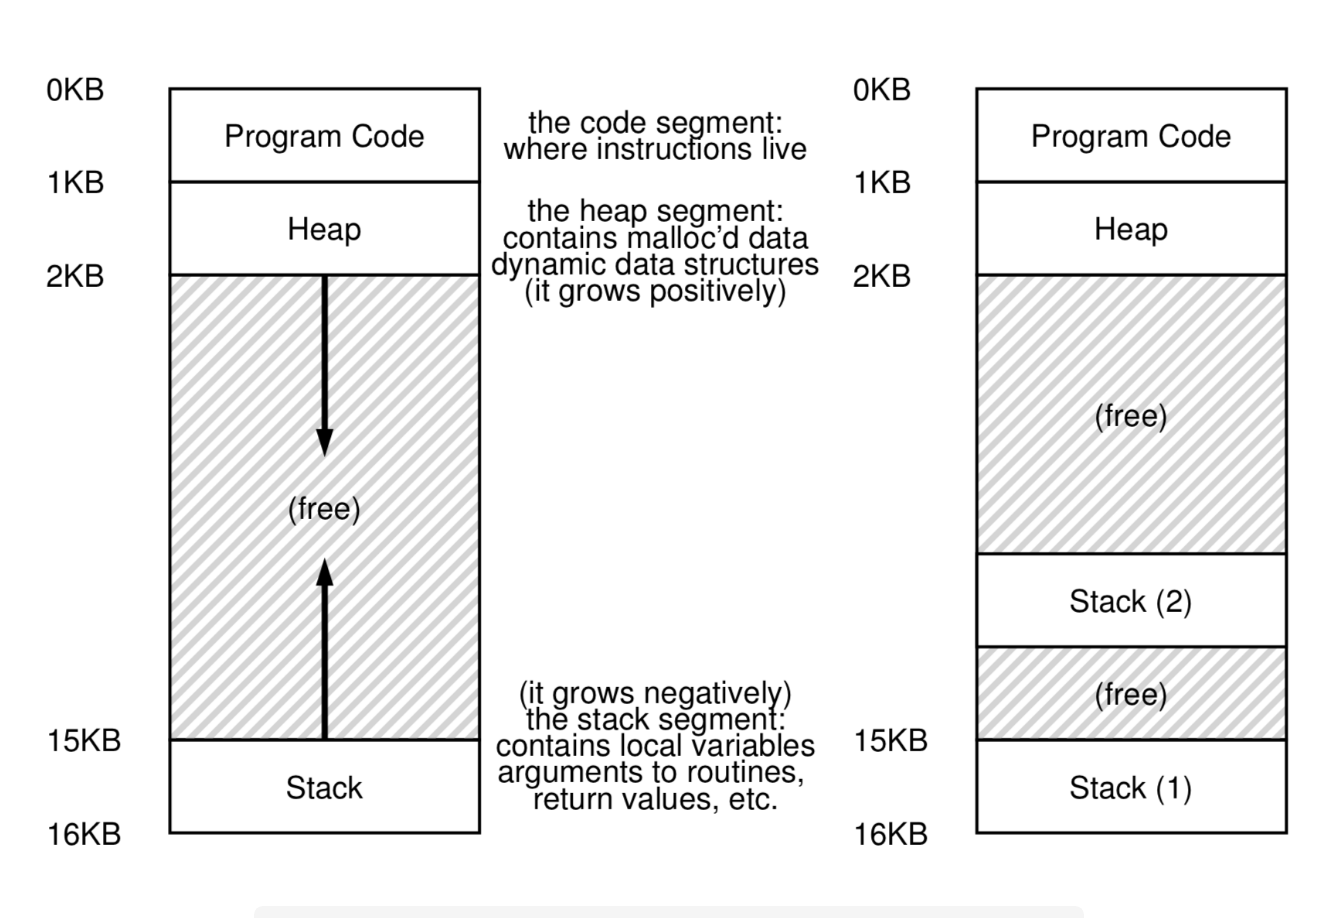
\includegraphics[width=0.65\textwidth]{chapters/Cucurrency/Cucurrency/ThreadAddressSpace.png}

\ssc{Benefit of using threads}

\sssc{Parallelism}

    Run works parallelly.

\sssc{Avoid Blocking}

    Avoid blocking program progress due to slow I/O; while one thread
    in the program waits, the CPU scheduler can switch to other ready threads.

    Threading enables overlap of I/O with other activities within a single program.

\sssc{Why not use processes instead?}

    Threads make it easy to share data, and often used to corporate with other threads
    to finish tasks.

    Processes are more sound choice for logically seperate tasks when little sharing
    of data structures in memory is needed.


\ssc{Problem with threads: Race Condition}

    \tbi{The execution sequence of threads is indeterministic}.

    Create two threads to update on the same global variable with the same function.
    
    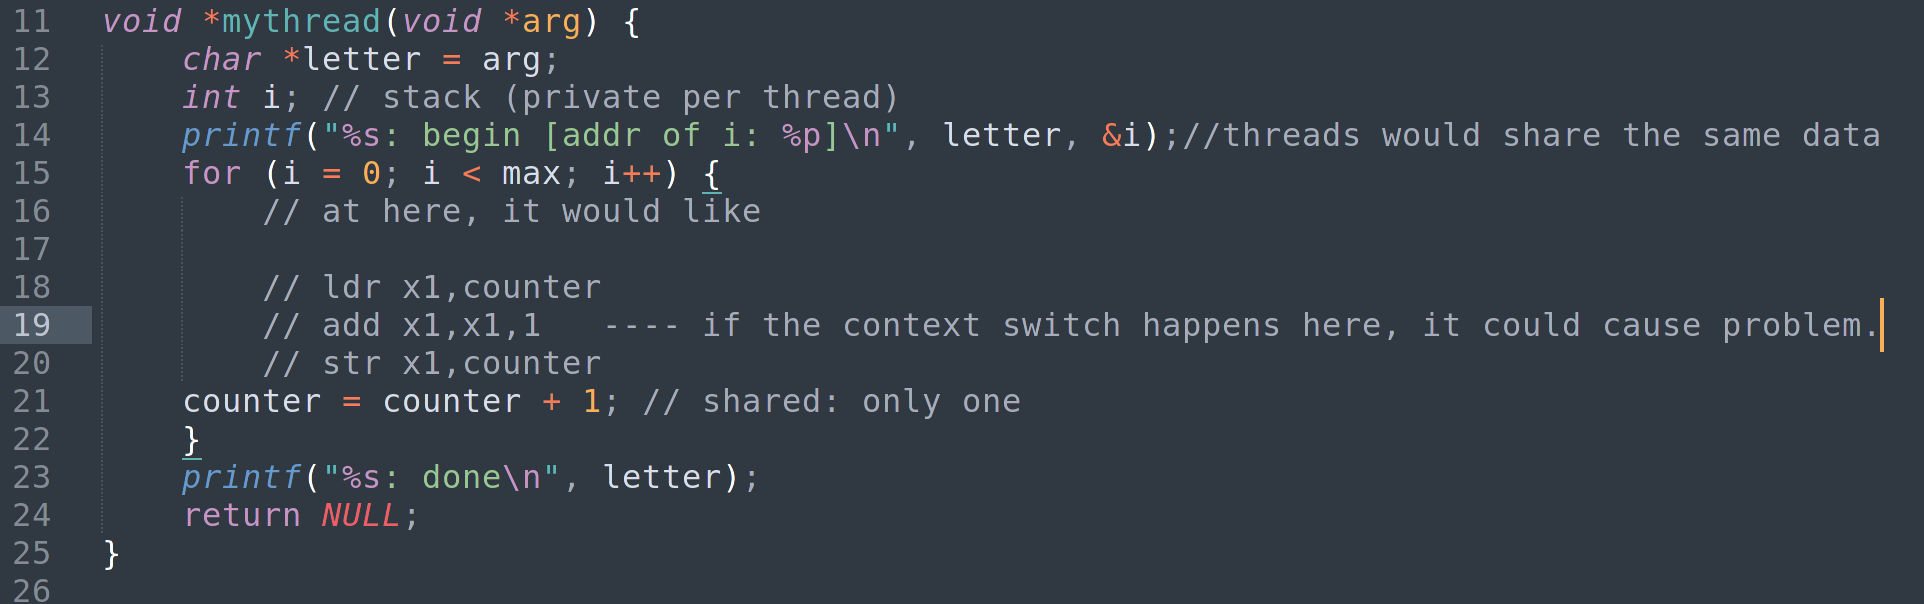
\includegraphics[width=0.75\textwidth]{chapters/Cucurrency/Cucurrency/thread_function.png}

    The problem can be:

    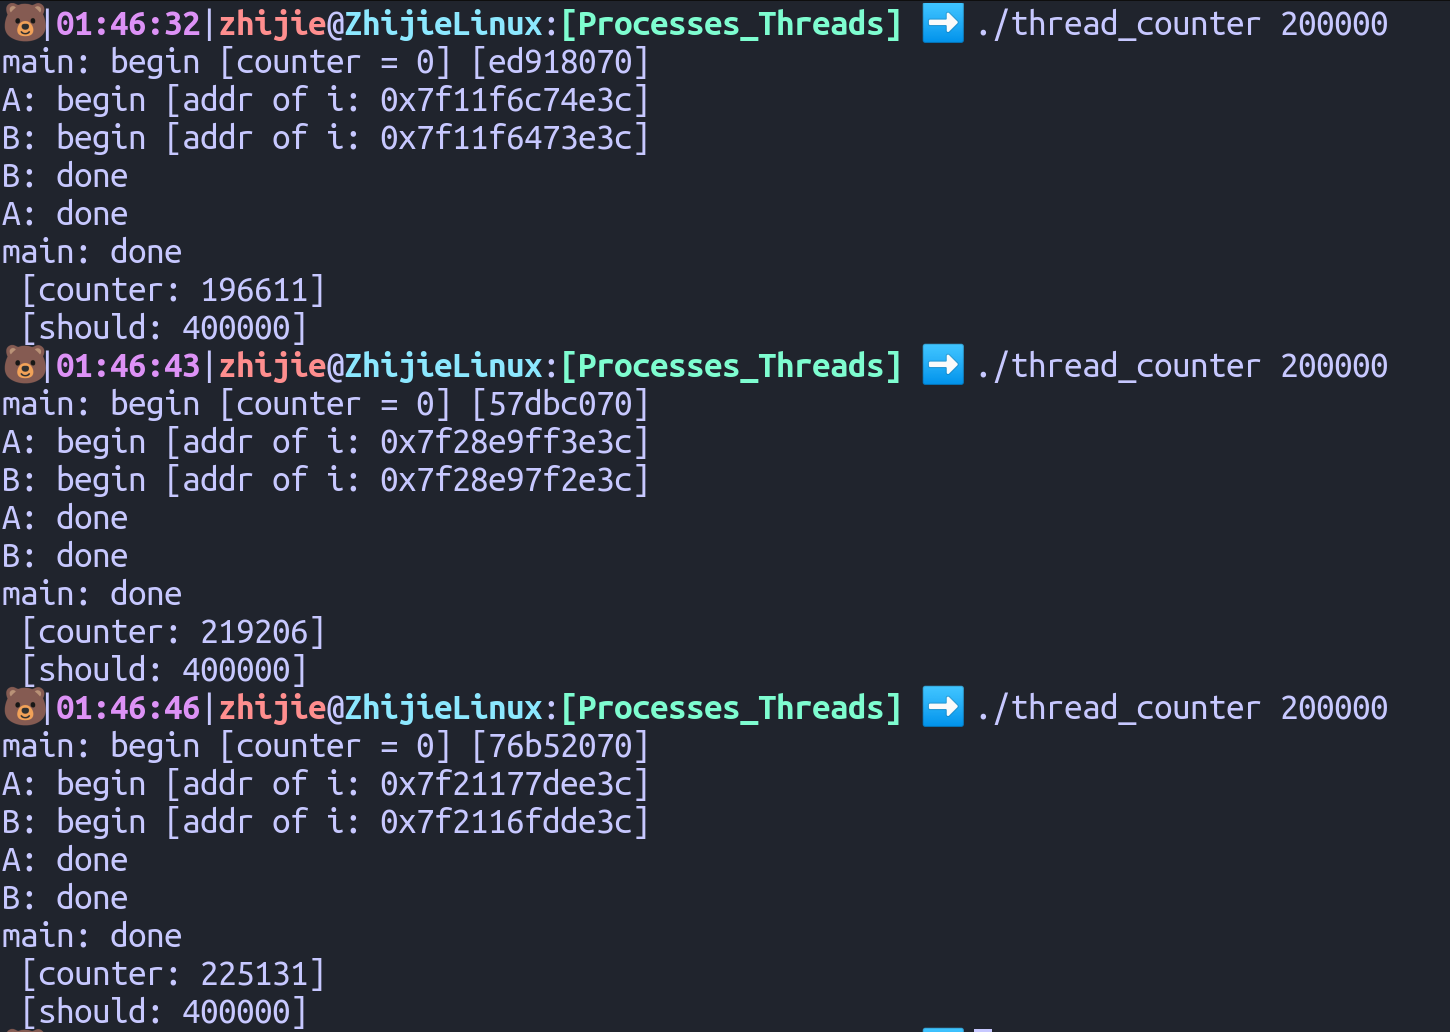
\includegraphics[width=0.7\textwidth]{chapters/Cucurrency/Cucurrency/thread_conflicts.png}


\sssc{Assembly Code}

    In ARMx8 Assembly:

    counter = counter + 1 is equivalent to 
    \begin{enumerate}
        \item ldr x1,[counter]
        \item add x1, x1, 1
        \item str x1, [counter]
    \end{enumerate}

\sssc{The work flow of causing problem}

    \begin{enumerate}
        \item Thread A loads counter into x1, say x1=50.
        \item Context switch happenes, and switch to Thread B.
        \item Now thread B loads counter into x1, x1=50.
        \item Thread B increase x1 by 1, x1=51.
        \item Thread B stores x1 back to counter, counter=51.
        \item Context switch happenes, and switch back to Thread A.
        \item Context Switch restores x1 for A,i.e, x1=50. And A won't load counter to x1 again
        \item Thread A increase x1 by 1, x1=51.
        \item Thread A stores x1 back to counter, counter=51.
        \item Thus, counter is set to 51 twice, although it should be 52 after the flow.
    \end{enumerate}

\sssc{Critical Section}

   \tbi{Critical Section}: A piece of code that accesses a shared variable, and
   must not be concurrenctly executed by more than one thread.
   
\sssc{Mutual Exclusion}

    \tbi{Mutual Exclusion:} if one thread is executing within the critical section, 
    the others will be prevented from doing so.

\sssc{Race Condition}

    Multiple threads of execution enter the critical section at roughly the same
    time; both attempt to update the shared data structure, 
    leading unexpected outcome.

\sssc{Atomicity}

    Atomic operation: grouped actions to be executed in one scheduling, i.e,
    the operation won't be interrupted.

    For example, x1 = x1 + x2 could be done in one single step with hardware support,
    instead of load, add, and store.

    It is desired to support atomicity for critical sections.   



\ssc{Thread API}

\sssc{Lock}
     
    In POSIX library, a lock needs to be initialized

    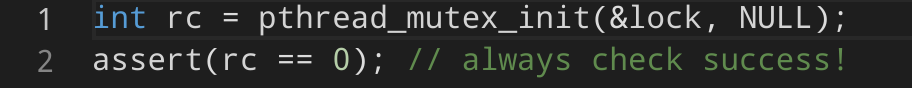
\includegraphics[width=0.6\textwidth]{chapters/Cucurrency/Cucurrency/init_lock.png}

    Also, a thread can acquire a lock, and release a lock.

    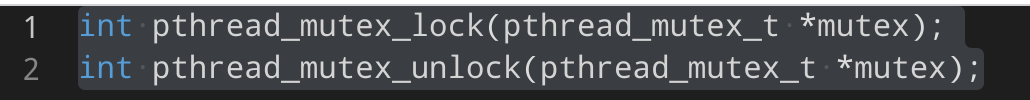
\includegraphics[width=0.6\textwidth]{chapters/Cucurrency/Cucurrency/lock_unlock.png}


\sssc{Condition Variable}

    Condition variables are useful when some kind of signaling must take place
    between threads if one thread is waiting for another to do something before it 
    continues.

    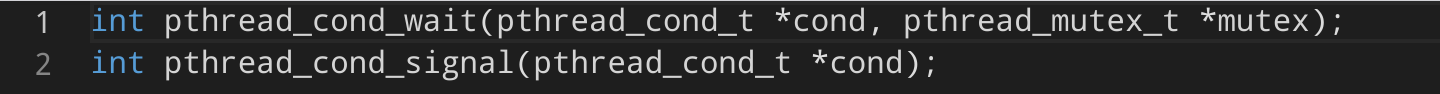
\includegraphics[width=0.6\textwidth]{chapters/Cucurrency/Cucurrency/condtion_wait_signal.png}

    A thread must hold a lock to call either wait() or signal(). 
    $pthread_cond_wait()$, puts the calling thread to sleep.
    $pthread_cond_signal()$ awakes the waiting thread.

    The reason that $pthread_cond_wait()$ takes two parameter is because
    it needs to specify which thread to give the lock to. When $pthread_cond_wait()$
    the calling thread release the lock and pass it to another thread.

\ssc{Locks and Building one}

\sssc{Basic}

    Lock is used around the critical section. It is a global variable that either 
    available or acquired and exactly one thread can hold it at a time.

    \tbi{mutex} in POSIX means \tbi{mutual exclusion} between threads.

\sssc{Evaluating Locks}

    Basic criteria:
    \begin{enumerate}
        \item Mutual exclusion: A lock must provide mutual exclusion, i.e, the lock
        should preventing multiple threads from entering a critical section.
        \item Fairness: Prevent starving a lock.
        \item Performance: How many overhead would be added to use the lock.
    \end{enumerate}

\sssc{Lock by Controlling Interrupts}

    One of the earliest implementation of lock is disable interrupts.

    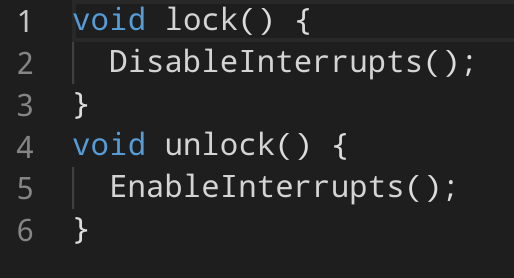
\includegraphics[width=0.6\textwidth]{chapters/Cucurrency/Cucurrency/earliest_lock.png}

    This approach works since it assumes mutual exclusion, and it is very simple.

    However, it has flaws:
    \begin{enumerate}
        \item Priviledged action: malicious process would disable the interrupts and
        never enable interrupts again.
        \item Interrupts would get lost: for example, I/O interrupts would get lost 
        and some processes which are waiting on those interrupts cannot move forward.
        \item Inefficient approach: It is very costly to enable/disable interrupts.
        \item No support for multiprocessors.
    \end{enumerate}

\sssc{A Fail Attempt: Using a Flag}

    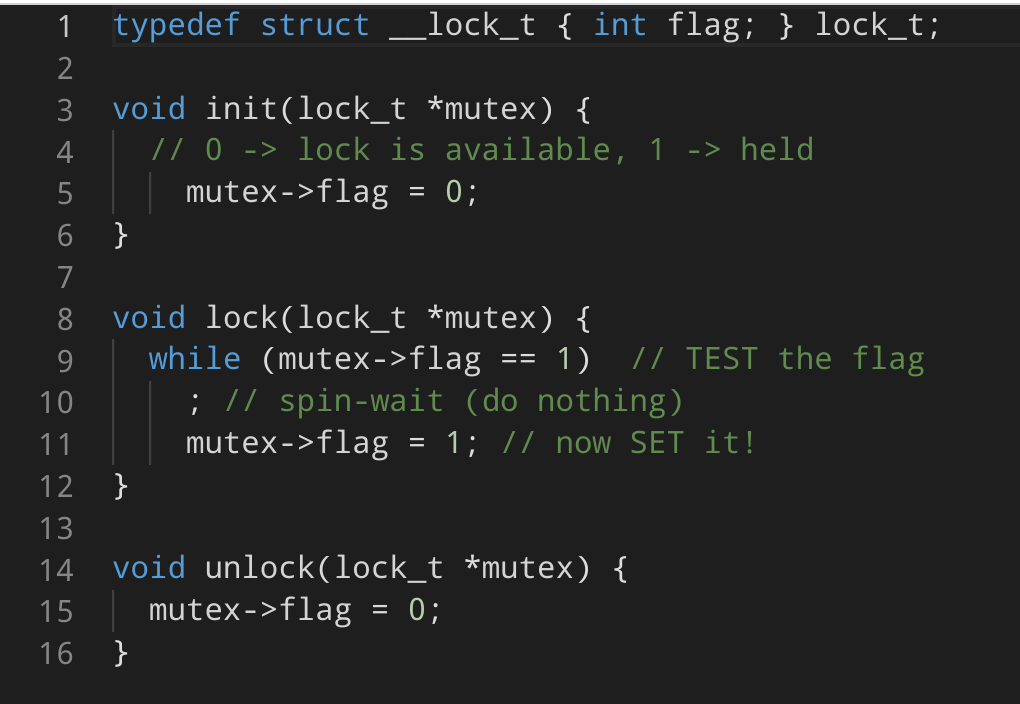
\includegraphics[width=0.6\textwidth]{chapters/Cucurrency/Cucurrency/lock_by_flag.png}

    \tbi{Correctness Problem}: Interleaving would give more locks than just one.

    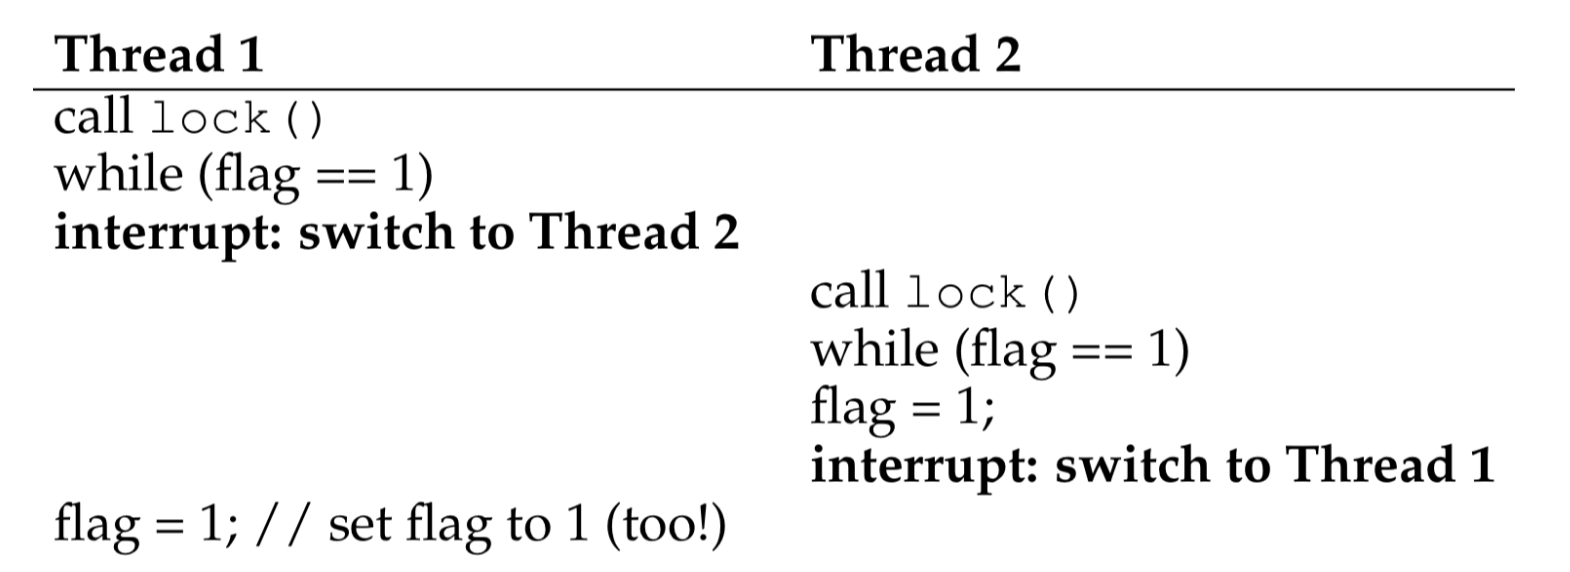
\includegraphics[width=0.6\textwidth]{chapters/Cucurrency/Cucurrency/Interleaving_problem.png}

    \tbi{Performance Problem}: While loops is valid instruction that would use CPU,
    it is very likely a thread which acquiring the lock spents its timeslot to 
    loop. This behavior is called \tbi{busy-waiting} or \tbi{spin-waiting}.

\sssc{Test-and-Set}

    \tbi{Test-and-Set} is atomic instruction supported by the hardware. It 
    both gets and sets the value in a register/address. 

    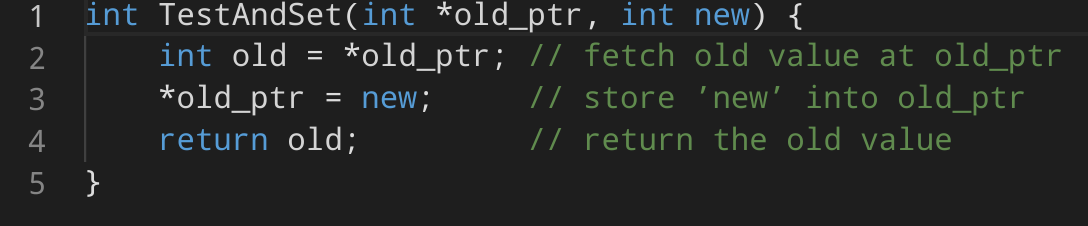
\includegraphics[width=0.6\textwidth]{chapters/Cucurrency/Cucurrency/test_and_set.png}

    With \tbi{Test-and-Set}, we can build a correct lock.

    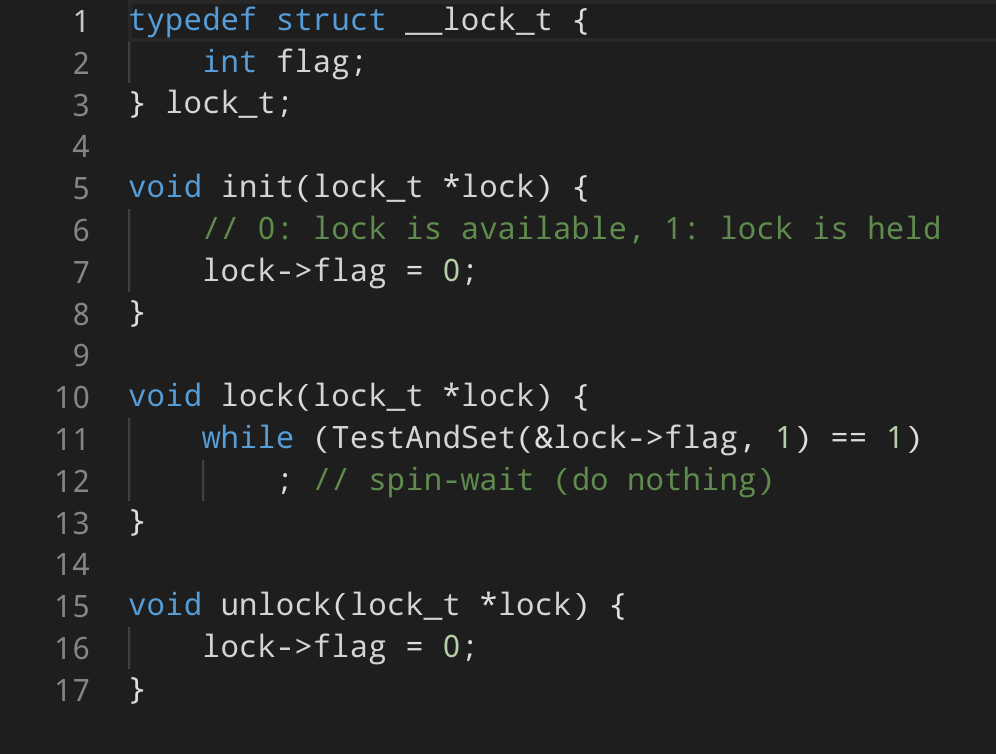
\includegraphics[width=0.7\textwidth]{chapters/Cucurrency/Cucurrency/spin_locks_test_set.png}

    However, the Test-and-Set approach doesn't guarantee
    \begin{enumerate}
        \item Fairness: There is no intelligence invoked to provide fairness.
        \item Performance: It is painful on a single CPU. Acceptable on multiple CPUs,
        because the CPU scheduler would switch the waiting thread out after its timeslot.
    \end{enumerate}

\sssc{Compare-And-Swap}

    \tbi{Compare-And-Swap}: Test whether the value equals; is so, 
    update the memory value. Finally,
    it would return the original value.

    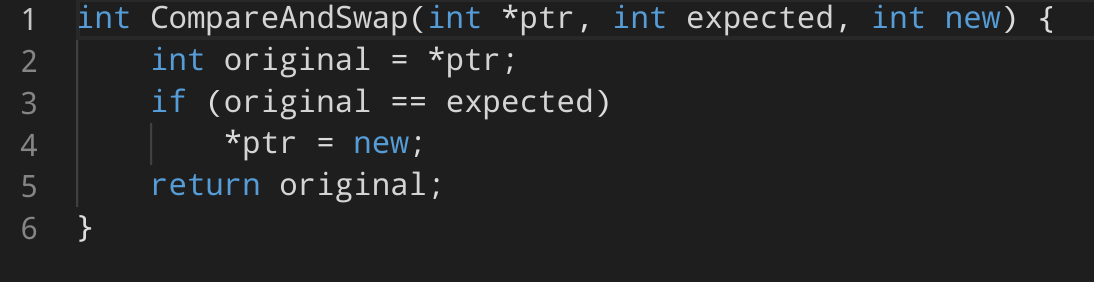
\includegraphics[width=0.65\textwidth]{chapters/Cucurrency/Cucurrency/compare_and_swap.png}

    With \tbi{Compare-And-Swap}, it is possible to build a spin clock

    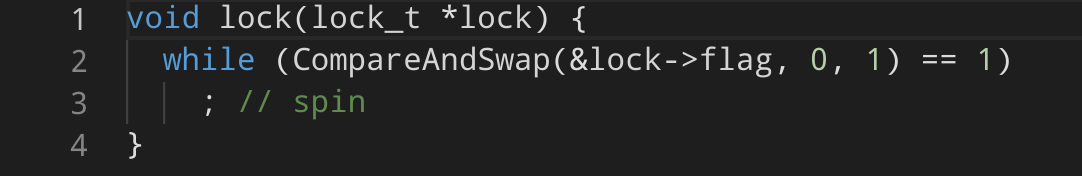
\includegraphics[width=0.65\textwidth]{chapters/Cucurrency/Cucurrency/compare_swap_spin_lock.png}

\sssc{Fetch-And-Add}

    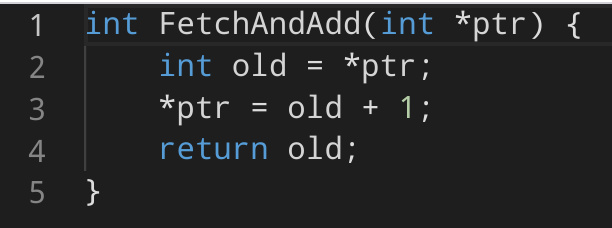
\includegraphics[width=0.6\textwidth]{chapters/Cucurrency/Cucurrency/fetch_and_add.png}

    And a spin clock can be build, a \tbi{ticket lock}

    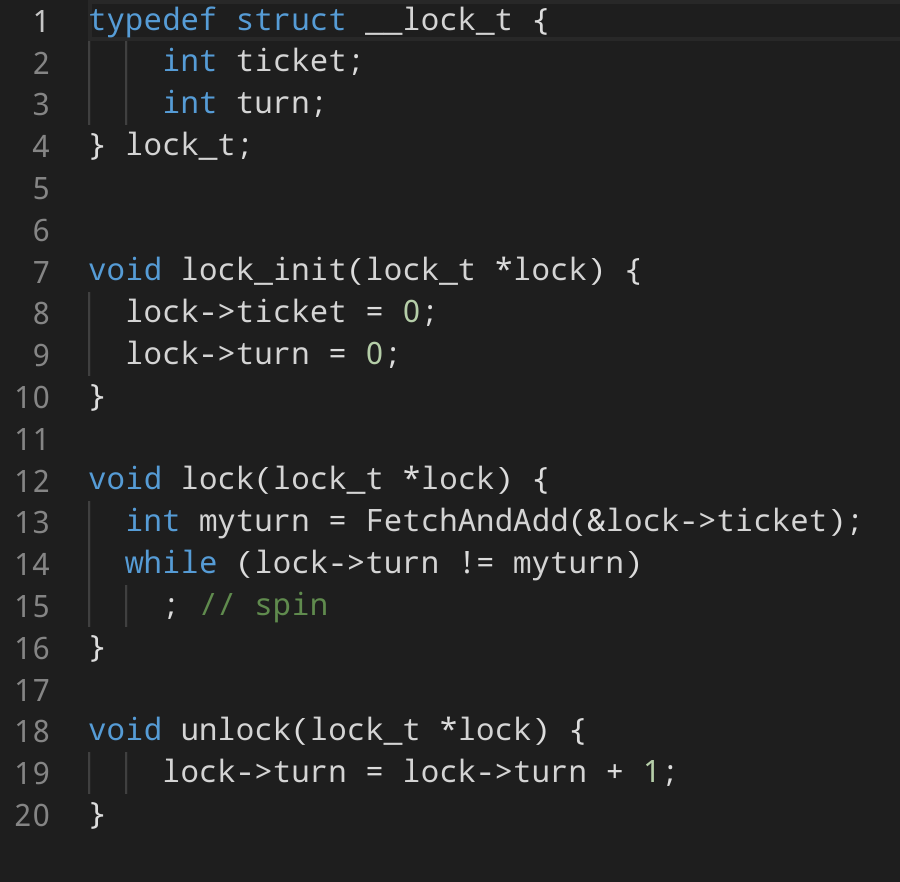
\includegraphics[width=0.6\textwidth]{chapters/Cucurrency/Cucurrency/ticket_lock.png}

    The advantage of \tbi{ticket lock} is that the approach "remeber" the requests of
    lock, i.e, it is like to pick a ticket that has number on it. And once the thread
    picks its ticket, all it needs to do is to wait and be called.

    $\Rightarrow$ this approach guarantees fairness.

    Other approaches are like fighting with each other for a single ticket.


\sssc{Spin locks and hardware limitation}

    With the extra hardware supports, we can now build spin locks. However the inefficiency is like 
    a diaster.

    Suppose each threads executes the same amount of time, with N threads and a single lock. The actual work
    done is $\frac{1}{N}$, and $\frac{N-1}{N}$ is useless busy-waiting.
    
    The hardware cannot solve everything, a smart software needs to be introduced in OS.

\sssc{Just yield, Baby}

    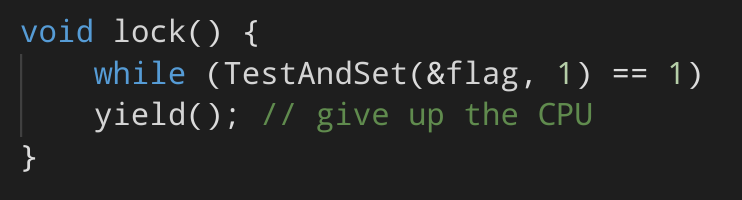
\includegraphics[width=0.5\textwidth]{chapters/Cucurrency/Cucurrency/yield.png}

    yield() is an operating system primitive which a thread can call when it wants to give up the CPU and 
    let another thread to run, i.e, descheduling the calling thread and move it from running to ready.

    
    \tbi{Efficiency Problem}:Suppose there are N threads and a single lock and the scheduler is taking round robin
    , N-1 yield would be called and only 1 critical section instruction would be executed. That is still 
    bad.

    \tbi{Fairness Problem}: If the scheduler is not using round robin, a thread would be picked consecutive to 
    call yield() which introduce the possibilty of starving a process.

\sssc{Using Queues: Sleeping Instead of Spinning}

    There are some controls needed over which thread next gets to acquire the lock after the current holder release
    it.

    Some OS support is need $\Rightarrow$ A queue to keep track of which threads are waiting to acquire the lock.

    \vspace*{2mm}
   
    \tbi{park()} and \tbi{unpark()}.

    In Solaris: \tbi{park()} to put a calling thread to sleep and \tbi{unpark(threadID)} to wake a particular
    thread as designated by \tbi{threadID}.

    When a thread tries to acquire the lock, the OS would park() to put the thread into sleeping and awakes it 
    by calling unpark(threadID) when the lock is free.

    
    \vspace*{2mm}
    
    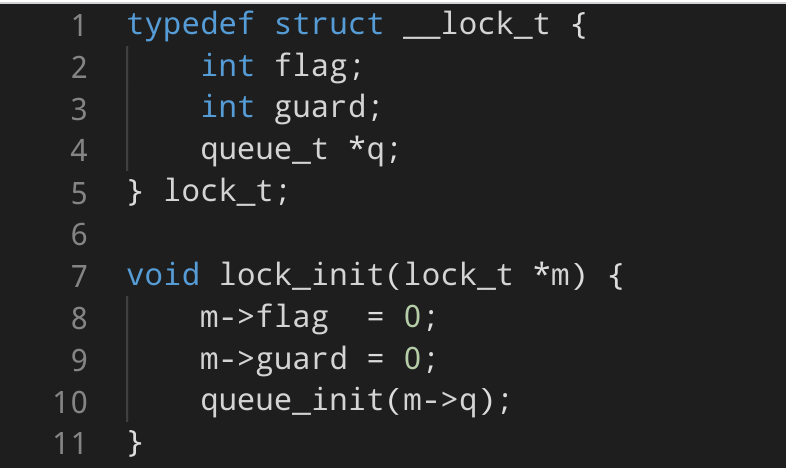
\includegraphics[width=0.6\textwidth]{chapters/Cucurrency/Cucurrency/lock_init.png}

    \tbi{Flag} indicates whether the lock is available, \tbi{guard} is used to ensure atomicity within 
    the lock()/unlock().

    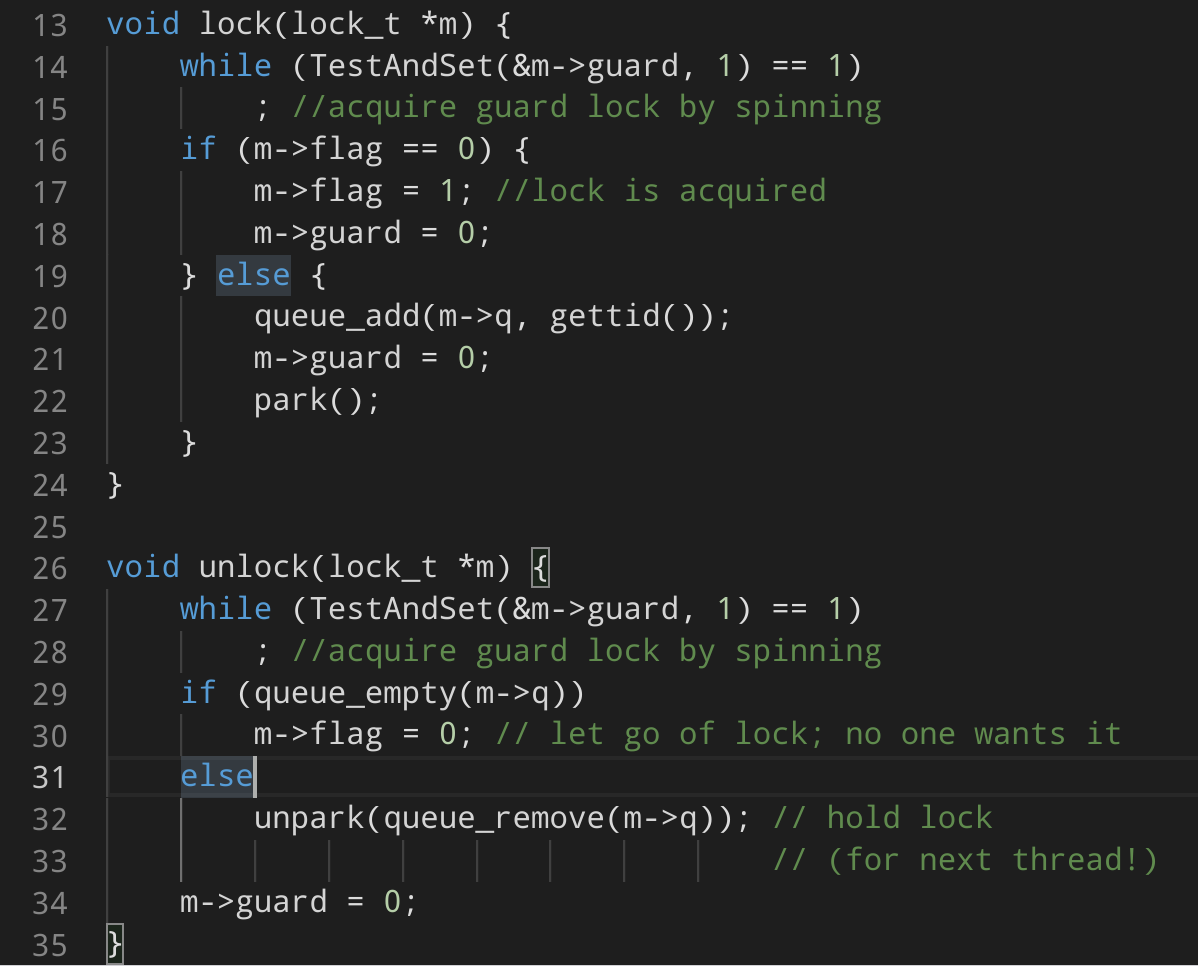
\includegraphics[width=0.7\textwidth]{chapters/Cucurrency/Cucurrency/park_unpark_approach.png}

    The guard is like another lock for the lock()/unlock(), one thread needs to hold the guard to acquire the 
    lock or put itself into sleep and release the guard.

    \vspace*{2mm}

    \tbi{Advantage:}
    \begin{enumerate}
        \item Small spinning/waste.
        \item Fairness by using the queue.
    \end{enumerate}

\sssc{Futex}

    A linux approach.... Kinda complicated, would take a look when studying linux.
    
    
    







